\documentclass{article}
\usepackage[paperwidth=8in,paperheight=4in,margin=0.1in]{geometry}
\pagestyle{empty}
\usepackage{amsfonts}
\usepackage{tikz}
\usetikzlibrary{positioning,calc,arrows.meta,decorations.pathreplacing,shadows,shapes.geometric,shapes.symbols}

% ==== Colors ====
\definecolor{frozenblue}{RGB}{100,150,200}
\definecolor{trainableyellow}{RGB}{255,200,100}
\definecolor{replaygreen}{RGB}{100,200,100}
\definecolor{outputpurple}{RGB}{200,100,200}
\definecolor{featgrey}{RGB}{230,230,230}

% ==== 3D Box style ( existing pic) ====
\tikzset{
  Box/.pic={
    \tikzset{/boxblock/.cd,#1}
    \tikzstyle{box}=[every edge/.append style={pic actions, densely dashed, opacity=.6},
                     fill opacity=\opacity, pic actions,fill=\fill]
    \pgfmathsetmacro{\y}{\cubey*\scale}
    \pgfmathsetmacro{\z}{\cubez*\scale}
    \pgfmathsetmacro{\x}{\cubex*\scale}
    \coordinate (a) at (0, \y/2, \z/2);
    \coordinate (b) at (0,-\y/2, \z/2);
    \coordinate (c) at (\x,-\y/2, \z/2);
    \coordinate (d) at (\x, \y/2, \z/2);
    \coordinate (e) at (\x, \y/2,-\z/2);
    \coordinate (f) at (\x,-\y/2,-\z/2);
    \coordinate (g) at (0,-\y/2,-\z/2);
    \coordinate (h) at (0, \y/2,-\z/2);
    \draw [box] (d) -- (a) -- (b) -- (c) -- cycle; % front
    \draw [box] (d) -- (e) -- (f) -- (c) -- cycle; % right
    \draw [box] (d) -- (a) -- (h) -- (e) -- cycle; % top
    \draw [box] (b) -- (g) -- (f) -- (c) -- cycle; % bottom
    \draw [box] (a) -- (h) -- (g) -- (b) -- cycle; % left
    \draw [box] (h) -- (e) -- (f) -- (g) -- cycle; % back
    \coordinate (\name-west)   at (0,0,0);
    \coordinate (\name-east)   at (\x,0,0);
    \coordinate (\name-north)  at (\x/2,\y/2,0);
    \coordinate (\name-south)  at (\x/2,-\y/2,0);
    \coordinate (\name-center) at (\x/2,0,0);
  },
  /boxblock/.search also={/tikz},
  /boxblock/.cd,
  width/.store in=\cubex,
  height/.store in=\cubey,
  depth/.store in=\cubez,
  scale/.store in=\scale,
  caption/.store in=\caption,
  name/.store in=\name,
  fill/.store in=\fill,
  opacity/.store in=\opacity,
  fill={rgb:red,5;green,5;blue,5;white,15},
  opacity=0.9,
  width=2,height=12,depth=14,scale=.25,
  caption=,name=,
}

\begin{document}
\centering
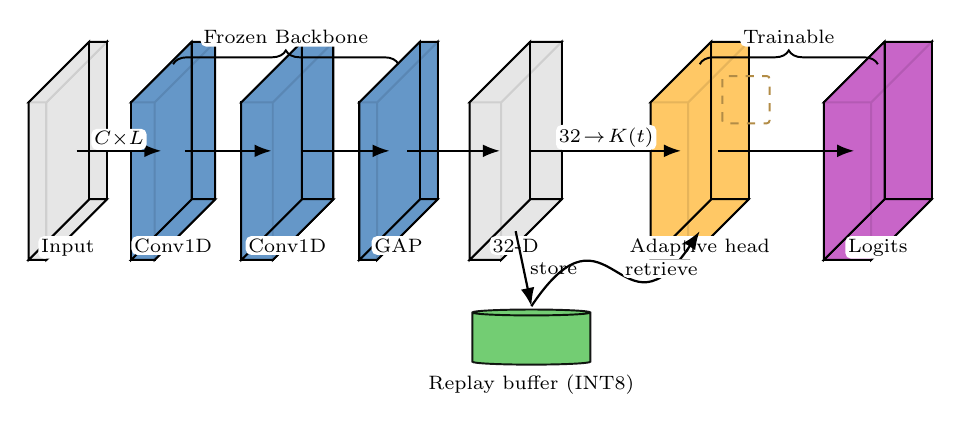
\begin{tikzpicture}[>=Latex, line width=0.7pt, font=\sffamily]

% small white-backed label
\tikzset{wb/.style={font=\scriptsize, fill=white, inner sep=1pt, rounded corners=2pt, text=black}}

% -----------------------------------------
% Compact backbone (frozen) — closer spacing
% -----------------------------------------
\pic at (-4.8,2.6) {Box={name=input,fill=featgrey,width=0.9,height=8,depth=8,scale=0.25}};
\node[wb,below=2pt of input-south] {Input};

\pic at (-3.5,2.6) {Box={name=conv1,fill=frozenblue,width=1.2,height=8,depth=8,scale=0.25}};
\node[wb,below=2pt of conv1-south] {Conv1D};

\pic at (-2.1,2.6) {Box={name=conv2,fill=frozenblue,width=1.6,height=8,depth=8,scale=0.25}};
\node[wb,below=2pt of conv2-south] {Conv1D};

\pic at (-0.6,2.6) {Box={name=gap,fill=frozenblue,width=0.9,height=8,depth=8,scale=0.25}};
\node[wb,below=2pt of gap-south] {GAP};

\pic at (0.8,2.6) {Box={name=feat,fill=featgrey,width=1.6,height=8,depth=8,scale=0.25}};
\node[wb,below=2pt of feat-south] {32-D};

% arrows + one dim label
\draw[->] (input-east) -- (conv1-west) node[midway,above,wb] {$C{\times}L$};
\draw[->] (conv1-east) -- (conv2-west);
\draw[->] (conv2-east) -- (gap-west);
\draw[->] (gap-east) -- (feat-west);

% frozen brace
\draw[decorate,decoration={brace,amplitude=5pt},yshift=6pt]
  ($(conv1-north)+(0,0.1)$) -- node[above=6pt,wb] {Frozen Backbone} ($(gap-north)+(0,0.1)$);

% -----------------------------------------
% Adaptive head (trainable) — minimal text
% -----------------------------------------
\pic at (3.1,2.6) {Box={name=head,fill=trainableyellow,width=1.9,height=8,depth=8,scale=0.25}};
\node[wb,below=2pt of head-south] {Adaptive head};

% small "grows" hint (very minimal)
\draw[dashed,trainableyellow!70!black,rounded corners=1pt]
  ($(head-east)+(0.05,0.35)$) rectangle ++(0.6,0.6);

\pic at (5.3,2.6) {Box={name=out,fill=outputpurple,width=2.4,height=8,depth=8,scale=0.25}};
\node[wb,below=2pt of out-south] {Logits};

\draw[->] (feat-east) -- (head-west) node[midway,above,wb] {$32 \!\rightarrow\! K(t)$};
\draw[->] (head-east) -- (out-west);

% trainable brace (compact)
\draw[decorate,decoration={brace,amplitude=5pt},yshift=6pt]
  ($(head-north)+(0,0.1)$) -- node[above=6pt,wb] {Trainable} ($(out-north)+(0,0.1)$);

% -----------------------------------------
% Replay buffer (INT8) — 3D cylinder, clearly labeled
% -----------------------------------------
\node[cylinder, draw=black, cylinder uses custom fill,
      shape border rotate=90,
      minimum width=1.5cm, minimum height=0.7cm,
      aspect=0.32, fill=replaygreen, opacity=0.9] (replay) at (1.2,0.2) {};
\node[wb,below=2pt of replay.south] {Replay buffer (INT8)};

% store / retrieve arrows (simple, readable)
\draw[->,thick] ($(feat-south)+(0,-0.02)$) -- ($(replay.north)+(0,0.03)$)
  node[midway,right=1pt,wb] {store};

\draw[->,thick] ($(replay.north)+(0,0.03)$) .. controls +(1.0,1.5) and +(-1.0,-1.5) .. ($(head-south)+(0,-0.02)$)
  node[midway,right=2pt,wb] {retrieve};
\end{tikzpicture}
\end{document}